\chapter{Project Context and Host Organization}

\section*{Introduction}
This chapter establishes the organizational and functional context of Qatra. It presents the host organization, clarifies the internship mission, analyzes the coordination problem, and identifies the stakeholders whose expectations shaped the platform.

\section{Keyrus Group}
Keyrus is an international consulting and technology group whose activities include data intelligence, digital experience, and business transformation. Its teams combine advisory work, systems integration, data engineering, software delivery, and operational support. This multidisciplinary positioning is aligned with Qatra because the project connects a social domain problem with software architecture, user experience, data consistency, DevOps, and observability concerns~\cite{keyrus}.

The group works through regional entities that combine local delivery with access to wider expertise. Engineering projects are approached as business transformations rather than isolated coding exercises: requirements, architecture, quality, deployment, and maintainability are considered throughout the delivery lifecycle.

\begin{figure}[H]
\centering

\includegraphics[width=0.62\textwidth,height=0.19\textheight,keepaspectratio]{assets/company/keyrus-ai-artwork.png}
\caption[Keyrus AI identity]{Keyrus AI identity and ``Architect of intelligence'' signature\\\emph{Source: artwork supplied for this report.}}
\end{figure}

\section{Keyrus MEA}
Keyrus MEA serves projects in the Middle East and Africa and collaborates with the wider Keyrus ecosystem. The internship environment exposed the project to enterprise delivery practices: explicit responsibilities, incremental planning, architectural justification, source control, automated workflows, and operational documentation. Qatra was developed as a coherent engineering product within this context, not as a disconnected prototype.

Figure~\ref{fig:keyrus-org} summarizes the organizational structure used in the reference company presentation. It situates the delivery teams beneath management and business-unit coordination without attributing Qatra to an unsupported internal department.

\begin{figure}[H]
\centering
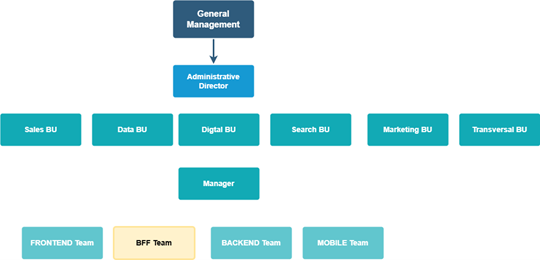
\includegraphics[width=0.92\textwidth]{assets/company/keyrus-org-chart.png}
\caption[Keyrus organizational structure]{Keyrus organizational structure adapted from the host-company material used in the reference report.}
\label{fig:keyrus-org}
\end{figure}

The host organization provided a setting in which backend, frontend, infrastructure, and reporting concerns could be treated together. This was important because a blood-donation platform cannot be evaluated only through isolated screens; reliability depends on the consistency of workflows across services and on the ability to observe them after deployment.

\section{Internship Mission}
The internship mission was to design and implement a distributed blood-donation and emergency-response platform. The work included:

\begin{itemize}
  \item analyzing donor, center, staff, and administrative workflows;
  \item defining functional and non-functional requirements;
  \item modeling the domain and its principal state transitions;
  \item implementing Spring Boot backend services and an Angular frontend;
  \item integrating persistence, security, asynchronous events, and real-time notifications;
  \item preparing Docker and k3s deployment resources;
  \item establishing CI/CD, monitoring, logging, and tracing configurations;
  \item documenting design decisions, validation evidence, and known limitations.
\end{itemize}

The mission required autonomy across several technical layers. It also required scope control: the purpose was to build a defendable platform foundation rather than claim integration with national health systems or operational blood inventories that were not part of the available project environment.

\section{Problem Statement}
Blood-donation coordination involves recurring and urgent needs. Recurring needs require centers to maintain a stable schedule of eligible donors. Emergencies require a focused response based on compatibility, distance, availability, and time. Donor suitability and donation testing remain medical responsibilities governed by qualified professionals and documented guidance, including the World Health Organization's donor-selection and blood-screening recommendations~\cite{whoDonorSelection,whoDonationTesting}. Traditional coordination mechanisms present several limitations:

\begin{itemize}
  \item donor records and availability may be fragmented or outdated;
  \item broad appeals notify people who are incompatible, unavailable, or too distant;
  \item appointment capacity and operating hours are not always visible to donors;
  \item staff must repeat administrative checks during check-in and screening;
  \item emergency progress is difficult to follow in real time;
  \item donors receive little feedback about eligibility, history, and impact;
  \item operational actions may lack a consistent audit trail.
\end{itemize}

The central question is therefore: \emph{how can a secure and maintainable digital platform coordinate donors, centers, appointments, emergencies, and notifications while keeping workflows traceable and responsive?}

\section{Study of Existing Solutions}
\subsection{General Coordination Approaches}
Existing approaches can be grouped into manual coordination, institutional portals, campaign-oriented applications, and integrated digital platforms. Table~\ref{tab:existing-approaches} summarizes their strengths and limits.

\begin{table}[H]
\centering\small
\begin{tabularx}{\textwidth}{|P{3.0cm}|Y|Y|}
\hline
\rowcolor{tableheader}\textbf{Approach} & \textbf{Strength} & \textbf{Typical limitation}\\ \hline
Telephone and spreadsheets & Familiar and inexpensive to start & Fragmented data, manual filtering, weak traceability, limited scalability\\ \hline
Institutional information portal & Authoritative center and campaign information & Often informational rather than transactional; limited personalization\\ \hline
Social-media emergency appeal & Rapid reach to a broad audience & No systematic eligibility, compatibility, distance, or response tracking\\ \hline
Standalone appointment application & Improves scheduling and reminders & May not cover emergencies, staff workflows, and cross-center administration\\ \hline
Integrated coordination platform & Unified donor, center, appointment, and emergency workflows & Requires stronger architecture, security, operations, and governance\\ \hline
\end{tabularx}
\caption{Comparison of blood-donation coordination approaches}
\label{tab:existing-approaches}
\end{table}

The critique supports an integrated approach but does not imply that every responsibility should be placed in one software component. Functional integration can coexist with technical modularity. Qatra therefore presents a unified user experience while separating principal backend responsibilities and using events for cross-service communication.

\subsection{Representative Digital Platforms}
To position Qatra against real services, this study examines five publicly documented platforms from Tunisia and other countries. Table~\ref{tab:existing-platforms} compares only capabilities described by their publishers. A feature that is not mentioned in the consulted material is treated as outside the published comparison, not as proof that the platform does not provide it.

\begin{longtable}{|P{3.0cm}|P{5.0cm}|P{5.4cm}|}
\hline
\rowcolor{tableheader}\textbf{Platform} & \textbf{Published capabilities} & \textbf{Position relative to Qatra's scope}\\ \hline
\endfirsthead
\hline
\rowcolor{tableheader}\textbf{Platform} & \textbf{Published capabilities} & \textbf{Position relative to Qatra's scope}\\ \hline
\endhead
CNTS Tunisia appointment platform & Online appointment booking for the national center in Tunis and the regional center in Sfax, intended to reduce waiting time, with extension to other regional centers announced~\cite{cntsplatform}. & Provides the most relevant local institutional reference. Qatra extends the study beyond appointment booking to donor profiles, center operations, emergency matching, notifications, analytics, and platform governance.\\ \hline
American Red Cross Blood Donor App & Finds nearby drives and centers, schedules and manages appointments, supports RapidPass, displays donation history and health information, and tracks a donation's journey~\cite{redcrossapp}. & Demonstrates a mature donor-centered experience. Qatra studies a broader multi-role workflow that also includes center staff, administrators, emergency coordination, and auditable operational actions.\\ \hline
NHS Give Blood & Shows nearby venues and real-time availability, manages appointments, presents donation history, blood group, milestones, and eligibility guidance~\cite{nhsgiveblood}. & Strong reference for appointment discovery and donor self-service. Qatra additionally focuses on urgent requests, compatibility-based candidate selection, response tracking, and center administration.\\ \hline
EFS Don de sang & Supports appointment booking, a donation suitability questionnaire, geolocation of nearby collection sites, personal information, and communication preferences~\cite{efsapp}. & Useful reference for accessibility and donor preparation. Qatra combines comparable donor services with staff workflows, emergency processing, notification delivery, and cross-center governance.\\ \hline
Facebook Blood Donations & Allows users to register for nearby blood-donation notifications and discover requests, blood banks, and donation events; Meta reported availability in Tunisia in 2021~\cite{facebookblood}. & Optimized for broad community reach and awareness. Qatra's design instead emphasizes verified platform roles, eligibility and compatibility checks, controlled emergency states, targeted delivery, and auditability.\\ \hline
\caption{Comparison of representative blood-donation platforms}
\label{tab:existing-platforms}
\end{longtable}

The comparison reveals two complementary tendencies. Institutional applications provide reliable appointment and donor-account services, while social platforms provide large-scale awareness and rapid dissemination. Qatra brings these concerns into one controlled domain model: appointments remain linked to center capacity, emergency alerts are filtered before dispatch, staff actions follow explicit states, and administrative operations are recorded. This positioning is a design objective of the project; it is not a claim of superior clinical or production performance.

\section{Proposed Solution: Qatra}
Qatra is a role-aware web platform centered on the donation lifecycle. A donor creates and verifies an account, completes profile and health information, sets location and availability, discovers centers, reserves a slot, completes screening, and receives a recorded donation outcome. Center staff manage daily operational tasks and authorized emergency workflows. Center administrators manage center information, slots, staff, activity, reports, and urgent requests within their scope. Super administrators govern users, center approvals, roles, audit records, and sensitive requests. The system filters and ranks eligible donors and dispatches notifications.

The platform context is summarized in Table~\ref{tab:system-context}. It identifies the principal actors, the Qatra boundary they use, and the information exchanged with the platform.

\begin{table}[H]
\centering\small
\begin{tabularx}{\textwidth}{|P{3.0cm}|P{4.2cm}|Y|}
\hline
\rowcolor{tableheader}\textbf{Actor} & \textbf{Qatra boundary} & \textbf{Principal interaction}\\ \hline
Donor & Donor and appointment workflows & Profile, health information, eligibility, availability, center discovery, booking, alerts, and responses\\ \hline
Center staff & Donation operations & Daily schedule, donor check-in, health screening, completion, and emergency coordination\\ \hline
Center administrator & Center governance & Center information, operating hours, slots, staff, activity, analytics, and reports\\ \hline
Super administrator & Platform governance & Users, roles, center approvals, restrictions, GDPR requests, dashboards, and audit records\\ \hline
\end{tabularx}
\caption{Qatra system context and principal stakeholders}
\label{tab:system-context}
\end{table}

\section{Project Stakeholders}
\begin{longtable}{|P{3.0cm}|P{4.1cm}|P{6.3cm}|}
\hline
\rowcolor{tableheader}\textbf{Stakeholder} & \textbf{Responsibility} & \textbf{Principal expectations}\\ \hline
\endfirsthead
\hline\rowcolor{tableheader}\textbf{Stakeholder} & \textbf{Responsibility} & \textbf{Principal expectations}\\ \hline
\endhead
Donor & Maintain profile, availability, appointments, and emergency responses & Simple onboarding, privacy, clear eligibility, useful reminders, accessible center information\\ \hline
Center staff & Execute check-in, screening, and appointment completion & Accurate daily schedule, fast access to authorized records, auditable actions\\ \hline
Center administrator & Operate a donation center and its team & Configurable slots, staff management, reports, activity visibility\\ \hline
Super administrator & Govern the platform & User and role control, center approval, audit and GDPR workflows\\ \hline
Company supervisor & Guide professional delivery & Visible progress, justified design, maintainable implementation\\ \hline
Academic supervisor & Guide academic quality & Traceable requirements, critical analysis, coherent validation\\ \hline
DevOps operator & Deploy and observe the platform & Repeatable releases, health information, logs, metrics, and rollback options\\ \hline
\caption{Qatra stakeholders and expectations}
\label{tab:stakeholders}
\end{longtable}

\section{Objectives and Constraints}
The principal objectives are to centralize donor and center workflows, reduce irrelevant emergency notifications, improve appointment coordination, preserve an audit trail, and provide an architecture that can evolve. The principal constraints are the sensitivity of health-related data, the need for role separation, asynchronous failure handling, geographical calculations, consistency across service boundaries, and the absence of direct integration with operational hospital systems in the project scope.

Success is therefore evaluated through coverage and coherence of implemented workflows, source-backed architecture, automated test presence, and operational configuration. It is not evaluated through unverified clinical impact or production usage figures.

\section*{Conclusion}
This chapter defined the professional context, the coordination problem, the stakeholders, and the boundaries of Qatra. The next chapter compares the architectural and technological alternatives that support these requirements.
